\documentclass[10pt,a4paper]{article}
\usepackage[margin=2.1cm]{geometry}
\usepackage[T1]{fontenc}
\usepackage{lmodern}
\usepackage{amsmath,amssymb}
\usepackage{graphicx}
\usepackage{booktabs}
\usepackage{tabularx}
\usepackage{multirow}
\usepackage{longtable}
\usepackage{array}
\usepackage{enumitem}
\usepackage{xcolor}
\usepackage[font=small,labelfont=bf]{caption}
\usepackage{float}
\usepackage[hidelinks]{hyperref}

\setlist{itemsep=1pt,topsep=2pt,parsep=0pt}
\setlength{\parindent}{0pt}
\setlength{\parskip}{4pt}
\graphicspath{{figures/}{../Question2/results/figures/}}
\newcommand{\figref}[1]{Figure~\ref{#1}}
\newcolumntype{Y}{>{\raggedright\arraybackslash}X}

\begin{document}

\begin{titlepage}
\centering
{\large Lahore University of Management Sciences}\\[2pt]
School of Science and Engineering, Department of Artificial Intelligence\\[14pt]
{\Large \textbf{AI651 -- Deep Learning for Space, Time and Graphs}}\\[6pt]
{\large Fall 2026 \quad\textbullet\quad Assignment 2}\\[40pt]
{\Large \textbf{Report}}\\[30pt]
\begin{tabular}{rl}
Student: & Danyal Tayyub \\
Roll number: & 24280023 \\
Code repository: & \url{https://github.com/danyaltayyub/DL4STG-PA2} \\
\end{tabular}
\vfill
\begin{minipage}{0.86\textwidth}
\small
\textbf{Contents.} Question~1 proposes a river-level forecasting system under the six required headings.
Question~2 trains a ConvLSTM forecaster on Moving MNIST, tests it under mirroring, rotation and speed-up,
separates appearance, unfamiliar-motion and reach failures with models B--D, and builds a symmetrised final
model. Code, GIFs and the pre-run predictions are in the repository (\texttt{Question2/}, \texttt{report/}).
The appendix lists the use of generative AI.
\end{minipage}
\vspace{20pt}
\end{titlepage}

\renewcommand{\thefigure}{Q1.\arabic{figure}}
\section{Question 1 --- River Forecasting Proposal}

\textbf{Proposal in one sentence.} A small, physics-shaped spatio-temporal graph network forecasts the
change in water level at S1--S4 over the next hour as quantiles. It routes upstream information along
the river graph with stage-dependent travel times, feeds announced reservoir releases in as known future
forcing, and adds the predicted change to the last observed level.

\subsection{Architecture diagram}

\begin{figure}[H]
\centering
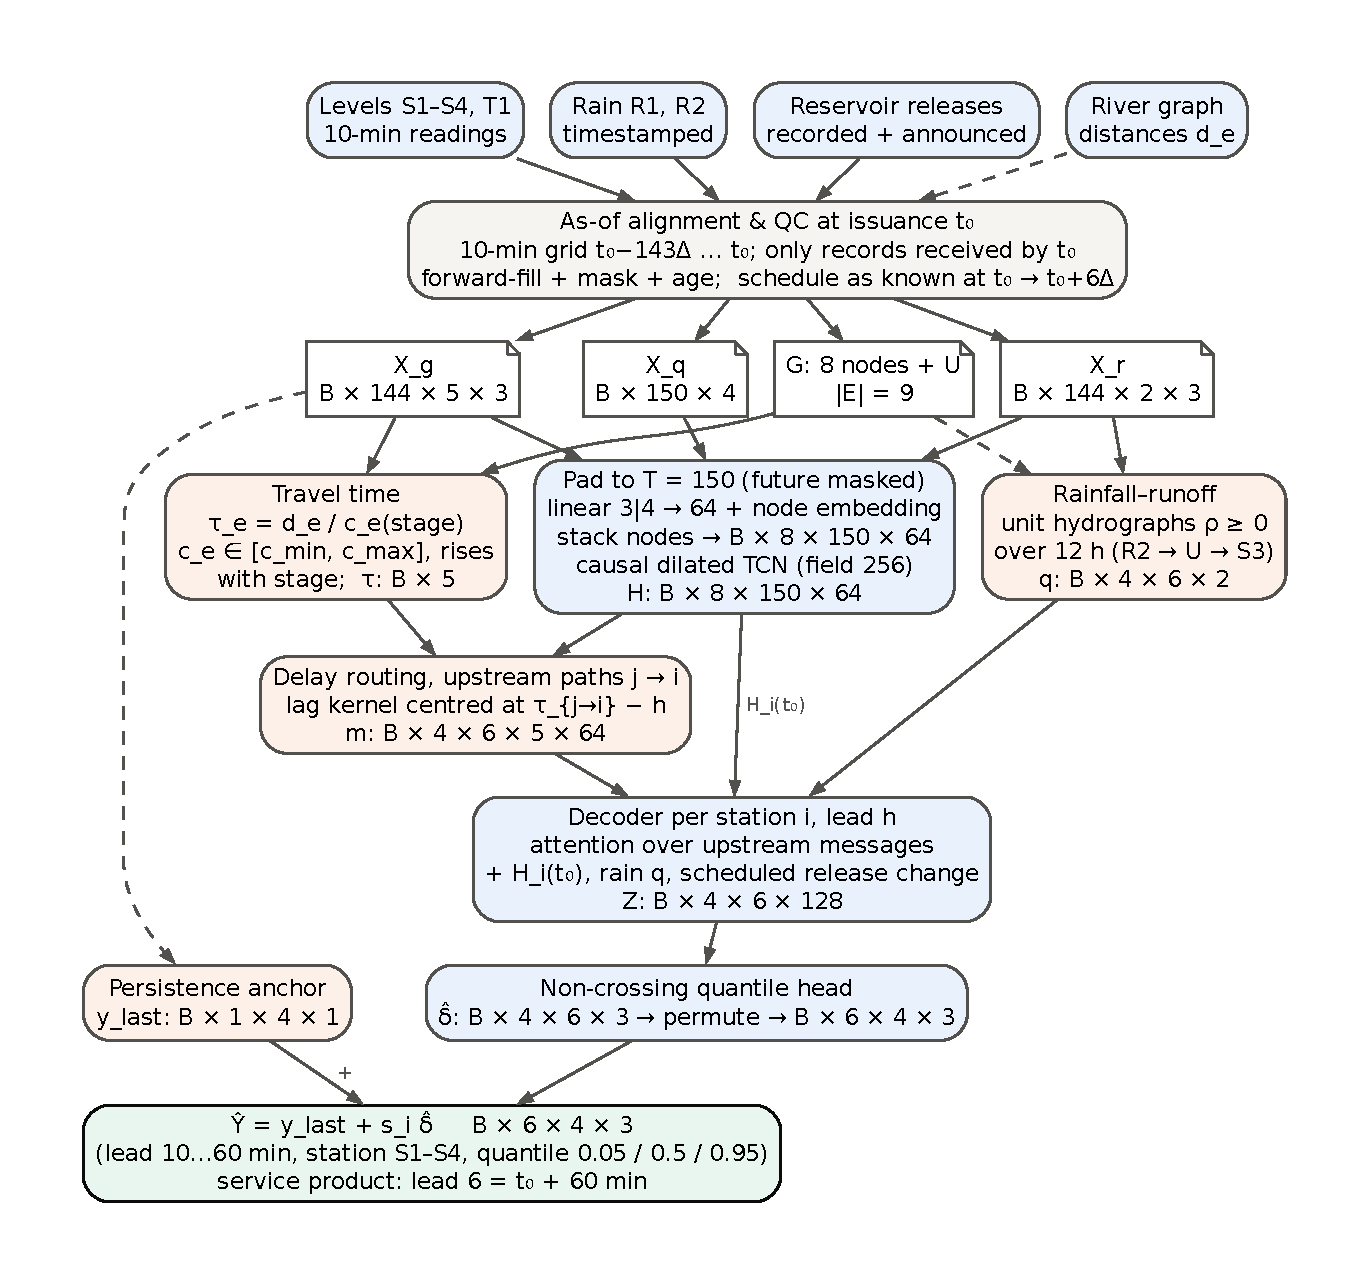
\includegraphics[width=0.93\textwidth]{q1_architecture.pdf}\\[2pt]
\begin{minipage}[c]{0.40\textwidth}
\centering
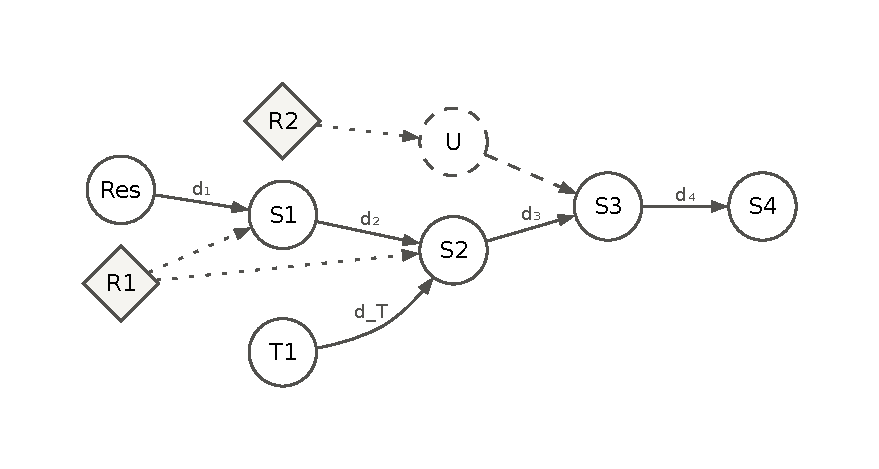
\includegraphics[width=\textwidth]{q1_river_graph.pdf}
\end{minipage}\hfill
\begin{minipage}[c]{0.57\textwidth}
\caption{Architecture (top) and the river graph used for routing (left). Blue blocks are learned networks;
orange blocks have a fixed physical form with a few learned parameters; note-shaped boxes are the input
tensors (axes are listed in the table of Section~\ref{sec:q1-task}). Forecasts are issued at $t_0$, and
$\Delta = 10$\,min. In the graph, solid arrows are channel reaches of length $d_e$, the dashed node $U$ is
the unmonitored tributary (no data; its inflow is inferred), and dotted arrows attach the rain gauges to
the catchments they represent.}
\label{fig:q1-arch}
\end{minipage}
\end{figure}

\subsection{Assumptions}

\textbf{Supplied facts.}
\textbf{F1}: 10-min water levels at S1--S4 and T1.
\textbf{F2}: rainfall at R1 and R2 with timestamps and gauge locations.
\textbf{F3}: recorded releases and schedules announced before issuance, with announcement and effective times.
\textbf{F4}: station locations, connectivity and along-river distances.
\textbf{F5}: travel times and the unmonitored tributary's inflow are not supplied; future rainfall and future
levels are unavailable at issuance.
Everything below is an \emph{assumption}, chosen to be the most defensible reading where the brief is silent.

{\small
\begin{longtable}{@{}p{0.04\textwidth}p{0.33\textwidth}p{0.25\textwidth}p{0.32\textwidth}@{}}
\toprule
ID & Assumption & Why it is reasonable & Effect on the design \\ \midrule
\endhead
A1 & All timestamps use one clock (stored in UTC). Readings are nominally every 10\,min with up to $\pm 2$\,min jitter. & Standard for telemetered gauges. & Every reading is assigned to the grid slot $(t-\Delta, t]$ that contains it (Section~\ref{sec:q1-task}). \\
A2 & Most records arrive within 5\,min, but outages can delay them by hours. Each record keeps its \emph{arrival} time. & Typical of radio/cellular telemetry. & Inputs are assembled \emph{as of} $t_0$ by arrival time, and a data-age feature marks staleness. Training replays arrival times (if they are not logged, see request I5). \\
A3 & At least 3 years of overlapping records exist, with several high-flow events and an archive of schedules \emph{as announced}. & The minimum for learning seasonal and event behaviour. & A small model (about $2\times10^5$ parameters) with physical structure. Train/validation/test split chronologically by year, with flood events in every split. \\
A4 & Level sensors are accurate to $\pm$1--2\,cm, with occasional spikes, flat-lines and logged datum shifts. Rain gauges are tipping buckets (0.2\,mm) that under-catch in wind. & Typical gauge specifications. & Range and rate-of-change checks turn bad values into missing values. The sensor noise sets the floor for useful accuracy. \\
A5 & Between stations, water only flows downstream; backwater at the confluences is negligible. & Steep mountain river (see the illustration). & Directed graph: a station only uses data from upstream nodes. \\
A6 & Travel time depends on the water level: higher water gives a faster flood wave (in-bank kinematic-wave behaviour), with mean velocities between 0.3 and 4\,m/s. & Standard open-channel hydraulics. & Each edge's wave speed $c_e$ is bounded and increases with stage, so its travel time is $d_e/c_e$. \\
A7 & Releases enter just above S1, and a release change reaches S1 within one hour. & S1 is directly below the dam in the map. & Scheduled releases inside the forecast hour act directly on S1, and on downstream stations when their path delay is short. \\
A8 & The unmonitored tributary is driven mainly by rain on its own catchment, which R2 (the nearest gauge) represents best; its baseflow varies slowly. & Gauge proximity in the map; baseflow changes over days. & Pathway R2 $\to U\to$ S3 through a rainfall--runoff kernel. Slow baseflow is absorbed by S3's own history. \\
A9 & R1 represents rain on the hillslopes between the dam and S2. T1 sits upstream of its confluence. & Gauge positions in the map. & R1 connects to every station from S1 down; T1 reaches S2 through edge T1$\to$S2 with its own delay. \\
A10 & Rain affects main-river levels after lags of 30\,min to 12\,h. The total reservoir-to-S4 travel time is under 12\,h. Snowmelt follows a daily cycle. & Small mountain catchment with snow (illustration). & A 24\,h history (144 steps) covers the longest lag and one full daily cycle. The encoder's receptive field is 256 steps. \\
A11 & Gaps can cluster during storms, because power and telemetry fail when flows are high. & Common in flood operations. & Training simulates outages that are concentrated on high-flow periods (Section~\ref{sec:q1-ops}). \\
A12 & Channel geometry, gauge datums and the reservoir's operating policy are stable over the record; slow drift is acceptable. & Needed to learn from history at all. & Periodic retraining plus drift monitoring; out-of-range stages are flagged. \\
\bottomrule
\end{longtable}
}

\subsection{Forecasting task and data specification}
\label{sec:q1-task}

\textbf{Issuance and horizon.} A forecast is issued every 10\,min at grid times $t_0$ (\texttt{hh:m0}), as soon
as the inputs have been assembled, typically within a minute of $t_0$. The \textbf{history window} is $L=144$
steps (24\,h), $t_0-143\Delta,\dots,t_0$, long enough for A10. The model predicts all six leads
$t_0+h\Delta$, $h=1,\dots,6$, jointly. This costs nothing extra, gives the intermediate leads as
supervision, and yields a trajectory for operators. The \textbf{service product} is $h=6$, the level at
$t_0+60$\,min at S1--S4, given as a median and a 90\% interval (quantiles 0.05, 0.5, 0.95).

{\small
\begin{longtable}{@{}p{0.09\textwidth}p{0.14\textwidth}p{0.36\textwidth}p{0.33\textwidth}@{}}
\toprule
Tensor & Shape & Axes and content & Timestamps / time coverage \\ \midrule
\endhead
$X_g$ & $B\times144\times5\times3$ & batch; history step; gauge (S1, S2, S3, S4, T1); [level as a per-station $z$-score, observed mask, data age in hours] & Slots $t_0-143\Delta,\dots,t_0$. Slot $t$ holds the latest reading timed in $(t-\Delta,t]$ that had arrived by $t_0$. \\
$X_r$ & $B\times144\times2\times3$ & batch; history step; rain gauge (R1, R2); [$\log(1+\text{mm})$ summed over the slot, mask, age] & Same slots. Future rain is unknown, so there are no future slots. \\
$X_q$ & $B\times150\times4$ & batch; 144 past + 6 future steps; [recorded release (scaled by capacity), scheduled release as known at $t_0$, recorded-value mask, is-future flag] & $t_0-143\Delta,\dots,t_0+6\Delta$. Past slots hold the actual and the then-scheduled rate; future slots hold the schedule from the latest announcement made by $t_0$. \\
$G$ & 8 data nodes + latent $U$; $|E| = 9$ & directed edges with lengths $d_e$ (km); node types (gauge, rain, reservoir) & Static. \\
$y^{\text{last}}$ & $B\times1\times4\times1$ & batch; --; S1--S4; last valid level in metres & The time of the last valid reading, which is $\le t_0$ (its age is in $X_g$). \\
$\hat Y$ (output) & $B\times6\times4\times3$ & batch; lead $h=1..6$; S1--S4; quantile (0.05, 0.5, 0.95); levels in metres above station datum & $t_0+10,\dots,t_0+60$\,min; served at $h=6$. \\
$Y$, $M_Y$ (training only) & $B\times6\times4$ & observed level at each lead, and a mask for missing targets & $t_0+h\Delta$, $h=1,\dots,6$. \\
\bottomrule
\end{longtable}
}

\textbf{Batch axis.} During training, $B$ is a set of issuance times sampled from the training years
(e.g.\ $B=256$). In operation $B=1$, or $B=2$ when a release scenario is run alongside (Section~\ref{sec:q1-ops}).

\textbf{Alignment across locations and sampling times.} All sources are put on one 10-min grid that ends at $t_0$:
\begin{itemize}
\item \textbf{Levels} snap to their slot (A1). An empty slot is forward-filled from the last valid value, with mask 0, and its age keeps growing.
\item \textbf{Rain} accumulations are summed per slot.
\item \textbf{Releases} are step functions sampled at slot times.
\item \textbf{Schedules} are \emph{as-of joined}: for each future slot, use the rate from the latest announcement whose announcement time is $\le t_0$.
\end{itemize}
Training uses the same rule, so the model never sees a schedule, reading or rain value it would not have had at $t_0$.
Uneven station spacing is not resampled away. It enters through the edge lengths $d_e$ and the travel-time
module, so each station is aligned with the \emph{lagged} state of its upstream nodes, not with their same-time state.
To combine sources in one encoder, gauge and rain inputs are padded with six masked future slots (a common axis, $T=150$),
projected per node type to 64 channels and stacked along the node axis: $B\times8\times150\times64$.

\textbf{Information available at issuance.} Everything that had arrived by $t_0$: levels and rain up to $t_0$,
releases recorded up to $t_0$ (possibly lagging), schedules announced up to $t_0$ (covering the future), and the
static graph. \emph{Not} available: future rain, future levels, schedule changes not yet announced, and the
unmonitored tributary's inflow.

\subsection{Model computations and design justification}

\textbf{Notation.} $\Delta=10$\,min, issuance time $t_0$, lead $h\in\{1,\dots,6\}$, hidden width $d=64$.
Nodes: reservoir $Q$, gauges $S_1$--$S_4$ and $T_1$, rain gauges $R_1$, $R_2$, and latent $U$ (no data).
$\mathrm{Up}(i)$ is the set of gauges and reservoir upstream of station $i$; the graph is a tree, so the path
$j\to i$ is unique. $\sigma$ is the logistic function, and $\mathrm{sp}$ is softplus.

\textbf{(1) Projection and encoder.} For node $j$ of type $\kappa(j)$ and slot $t$:
$e_j(t)=W^{\kappa(j)}x_j(t)+p_j$, where $p_j$ is a learned node embedding. Then 8 residual causal
dilated convolution layers (kernel 2, dilation $2^\ell$) are applied:
\[
H^{(\ell+1)}_j(t)=H^{(\ell)}_j(t)+\mathrm{GELU}\big(W^{(\ell)}_0H^{(\ell)}_j(t)+W^{(\ell)}_1H^{(\ell)}_j(t-2^\ell\Delta)\big),\qquad H_j=H^{(8)}_j\in\mathbb R^{150\times d}.
\]
Causality means $H_j(t)$ only depends on inputs at slots $\le t$. In the future slots, the reservoir carries the
announced schedule, and gauges and rain carry only ``unobserved'' tokens.

\textbf{(2) Travel time (physical form, learned parameters).} For edge $e=(j\to k)$, with $\bar y_j$ and $s_j$ the
training mean and standard deviation of station $j$'s level:
\[
c_e = c^{\min}_e+(c^{\max}_e-c^{\min}_e)\,\sigma\!\big(\mathrm{sp}(\alpha_e)\,(y^{\text{last}}_j-\bar y_j)/s_j+\beta_e\big),\qquad
\tau_e=\frac{d_e}{c_e\,\Delta},\qquad \tau_{j\to i}=\sum_{e\in \mathrm{path}(j,i)}\tau_e .
\]
$c_e$ is bounded (A6) and increases with stage, because $\mathrm{sp}(\cdot)\ge0$. The travel times $\tau$ are
measured in steps and can be read off for checking against hydrological knowledge.

\textbf{(3) Delay routing.} Upstream water that reaches station $i$ at $t_0+h\Delta$ passed node $j$ about
$\tau_{j\to i}$ steps earlier, i.e.\ $k^\star=\tau_{j\to i}-h$ steps before $t_0$. Let $k\in\{-6,\dots,143\}$
count steps before $t_0$ (negative values are future slots). Then:
\[
\kappa_{ji,h}(k)=\frac{\exp\!\big(-(k-k^\star)^2/2\varsigma_{ji}^2\big)}{\sum_{k'}\exp\!\big(-(k'-k^\star)^2/2\varsigma_{ji}^2\big)},\qquad
m_{ji,h}=\sum_k\kappa_{ji,h}(k)\,H_j(t_0-k\Delta),\qquad \phi_{ji,h}=\sum_{k<0}\kappa_{ji,h}(k).
\]
$\varsigma_{ji}=\mathrm{sp}(\cdot)$ is a learned spread that represents wave dispersion (Muskingum-like attenuation).
$\phi_{ji,h}$ is the share of the kernel that falls in the future. For the reservoir, those slots hold the
\emph{announced schedule}, so a release change reaches each station after its physical delay. For a gauge they
hold no data, so $\phi$ tells the decoder that this upstream signal has not arrived yet; the decoder then leans
on nodes further upstream, whose delays are longer.

\textbf{(4) Rainfall--runoff.} Each rain gauge $r$ connects to every station downstream of where it attaches
(R1: S1--S4; R2, through $U$: S3, S4), using a non-negative 12\,h unit hydrograph:
\[
q_{ri,h}=\sum_{\ell=0}^{71}\rho_{ri}(\ell)\,R_r\big(t_0+h\Delta-\ell\Delta\big),\qquad \rho_{ri}(\ell)=\mathrm{sp}(\theta_{ri\ell})\ge0,\qquad R_r(t>t_0)=0 .
\]

\textbf{(5) Decoder and forecast mapping.} Query $u_{i,h}=W_q[H_i(t_0);p_i;\eta_h]$, where $\eta_h$ is a lead
embedding. Each upstream source contributes the key $k_{ji,h}=W_k[m_{ji,h};\tau_{j\to i};\phi_{ji,h}]$:
\[
a_{ji,h}=\operatorname*{softmax}_{j\in\mathrm{Up}(i)}\!\big(u_{i,h}^{\top}k_{ji,h}/\sqrt d\big),\qquad
z_{i,h}=\mathrm{MLP}\big([u_{i,h};\textstyle\sum_j a_{ji,h}W_vk_{ji,h};q_{\cdot i,h};\delta^{Q}_h]\big)\in\mathbb R^{128},
\]
where $\delta^Q_h$ is the scheduled change in release between $t_0$ and $t_0+h\Delta$. The head
$(o_1,o_2,o_3)=W_oz_{i,h}$ gives quantiles of the standardised change that cannot cross:
\[
\hat\delta^{0.5}=o_1,\quad \hat\delta^{0.05}=o_1-\mathrm{sp}(o_2),\quad \hat\delta^{0.95}=o_1+\mathrm{sp}(o_3),\qquad
\hat Y^{(q)}_{h,i}=y^{\text{last}}_i+s_i\,\hat\delta^{q}_{i,h}.
\]

\textbf{(6) Training objective.} A masked pinball loss, weighted towards the service lead ($w_6=2$, $w_{1..5}=1$),
plus a smoothness penalty on the unit hydrographs:
\[
\mathcal L=\frac{\sum_{b,h,i}M_{Y,bhi}\,w_h\sum_{q}\rho_q\big(Y_{bhi}-\hat Y^{(q)}_{bhi}\big)}{\sum_{b,h,i}M_{Y,bhi}\,w_h}
+\lambda\sum_{r,i,\ell}\big(\rho_{ri}(\ell{+}1)-2\rho_{ri}(\ell)+\rho_{ri}(\ell{-}1)\big)^2,\qquad
\rho_q(u)=\max(qu,(q-1)u).
\]
Training uses AdamW with early stopping on the validation pinball loss at $h=6$, and random input masking
(Section~\ref{sec:q1-ops}). Interval widths are then calibrated per station on the validation years
(split-conformal adjustment), so the 90\% band covers about 90\%.

\textbf{Why these choices.}
\begin{itemize}
\item \emph{Predict the change, anchored on the last level.} Over one hour, persistence is the strongest simple
forecast. Learning the change removes datum differences between stations and leaves the network the dynamics.
\item \emph{Explicit travel-time routing instead of stacked message passing.} With $K$ message-passing layers,
information only travels $K$ hops, and it must also arrive at the right \emph{lag}. On a 4-hop chain, routing
along each upstream path gives full reach in hops and in time in one step, with a handful of parameters per
edge. Travel times that change with conditions (A6) are modelled directly instead of being averaged away.
\item \emph{Causal dilated convolutions instead of temporal attention.} A 256-step receptive field costs linear
time and memory. Attention would cost $O(L^2)$, and its main benefit, finding the relevant lag, is already
provided by the routing kernel.
\item \emph{Non-negative unit hydrographs.} More rain can never lower the forecast, and a linear kernel can be
learned from few storms.
\item \emph{Quantile outputs.} Flood preparedness needs risk, e.g.\ $P(\text{S4}>\text{threshold})$, not just a
point value.
\end{itemize}

\textbf{How each driver reaches each forecast.}
\begin{itemize}
\item \textbf{S1}: its own history; the reservoir's recorded and announced releases, with a short delay
(announced changes within the hour matter most); rain at R1.
\item \textbf{S2}: adds S1 and T1, each through its own delay; the reservoir through the path
$Q\to$ S1 $\to$ S2; R1.
\item \textbf{S3}: adds S2 and everything upstream of it. The \emph{unmonitored tributary} enters in two ways:
R2's rainfall--runoff kernel, and S3's own history, whose departure from routed S2 is a running proxy for the
tributary's inflow.
\item \textbf{S4} (next to the town): all of the above through S3 and the longer paths. For short leads, S3's
recent state dominates.
\end{itemize}

\textbf{Physical assumptions versus learned mappings.}
\begin{itemize}
\item \emph{Physical, fixed by design:} graph topology and flow direction, edge lengths, travel time
$=$ distance / wave speed, wave-speed bounds that increase with stage, causal and as-of masking,
non-negative rain response, the persistence anchor, and announced releases entering only through path delays.
\item \emph{Learned:} the wave-speed curves, dispersion, unit hydrographs, encoder, attention, decoder and quantiles.
\end{itemize}
A separate hydraulic simulator is not needed: the physics enters through structure and constraints. A simulator's
output could later be added as one more input node (request I2).

\subsection{Operation and exceptional conditions}
\label{sec:q1-ops}

\textbf{(i) Missing observations.}
\begin{itemize}
\item Missing or quality-rejected values are forward-filled with mask 0 and a growing age, never set to zero, so
input scales stay meaningful.
\item If a station's own reading at $t_0$ is missing, $y^{\text{last}}$ is its last valid value, and the age
feature lets the network widen its intervals and rely on upstream nodes.
\item During training, inputs are randomly masked: single slots, runs of up to 6\,h, and whole-station outages
concentrated on high-flow periods (A11). Missing targets are excluded through $M_Y$.
\item A station whose data are older than 6\,h is flagged ``degraded'' on the dashboard. Its forecast is still
issued, from upstream routing plus its last value.
\end{itemize}

\textbf{(ii) Delayed observations.}
\begin{itemize}
\item Inputs are assembled by \emph{arrival} time (A2). A late reading is invisible to the forecasts issued
before it arrives, and is used automatically from the next issuance on.
\item The model keeps no state between runs (each forecast is recomputed from the 24\,h window), so late data
never corrupt a carried-over state.
\item Training replays the logged arrival times, so the network sees the same kind of staleness it meets in
operation.
\end{itemize}

\textbf{(iii) Announced future releases.}
\begin{itemize}
\item These are \emph{known future inputs}. Each forecast uses the latest announcement made by $t_0$, as-of
joined onto the future slots of $X_q$, and they act through the routing delays ($\phi>0$ for the reservoir).
\item If no announcement covers the hour, the current rate is assumed to continue, and a flag is set.
\item Announcements made \emph{after} $t_0$ are never used, either in training or in operation.
\end{itemize}

\textbf{(iv) Differences between scheduled and actual releases.}
\begin{itemize}
\item Past slots of $X_q$ hold both the recorded and the then-scheduled rate. The network therefore learns how
reliably schedules are followed, and widens its intervals when recent deviations are large.
\item Once a deviation is recorded, it replaces the schedule for those past slots at the next issuance.
\item For operators, a second scenario is run in the same batch ($B=2$: ``as scheduled'' and ``current rate
continues''). The spread between the two shows how sensitive each station is to the release decision.
\end{itemize}

\textbf{Feasibility every 10 minutes.} The model has about $2\times10^5$ parameters. One forecast is a single
forward pass over $8\times150$ node-steps, on the order of $10^7$ multiply-adds: milliseconds on one CPU core.
Assembling 24\,h of records is a few small database queries. A run therefore takes seconds, far inside the
10-minute cycle, which leaves room for scenario runs, an ensemble of seeds and retries. If the model service
fails, persistence plus routed upstream change is issued as a fallback and labelled as such.

\subsection{Uncertainty, limitations, and additional information}

{\small
\begin{longtable}{@{}p{0.2\textwidth}p{0.36\textwidth}p{0.38\textwidth}@{}}
\toprule
Item & Forecast impact & Response, or what remains unresolved \\ \midrule
\endhead
Unmonitored tributary & Its inflow is invisible. This mainly affects S3 and S4 during local storms on its catchment. & Inferred from R2's kernel and S3's departure from routed S2, with wider quantiles when R2 is raining. \emph{Unresolved:} storms that R2 misses, and the size of the inflow from rain falling within the hour. \\
Changing travel times & Wrong timing of a flood wave gives the largest errors on the rising limb. & Wave speed depends on stage, within physical bounds, and travel times are checked against observed event lags. \emph{Unresolved:} over-bank flow at record floods can slow the wave, outside the training range; such stages are flagged. \\
No future rainfall & Rain falling in the next hour on hillslopes near S1/S2 is not in the inputs, so rapid rises are under-forecast. & Quantiles widen with current rain intensity. Fully fixed only by nowcasts (I3). \\
Release deviations & An unannounced change shows up first at S1 and then propagates downstream. & Deviation features and the two-scenario output (Section~\ref{sec:q1-ops}). \\
Data gaps in storms & Fewer inputs exactly when accuracy matters most. & Masking-robust training, degraded flags and persistence fallback. Remaining risk: large gaps at S3/S4. \\
Rare extremes & Few large floods to learn from, so the highest stages extrapolate. & Physical structure, a small model, held-out events for testing, and conformal calibration. Not fully resolvable without longer records. \\
Levels instead of discharge & Inflows do not add up in level units, so no mass balance can be imposed. & The level response is learned (non-linear decoder). Resolved by rating curves (I1). \\
Sensor drift / datum shifts & Bias at one station that propagates downstream. & Quality-control rules, a residual monitor against routed upstream levels, and retraining after logged datum changes. \\
Snowmelt and non-stationarity & Daily melt cycles and changing operating policies shift the input--output relation. & The 24\,h window includes yesterday's cycle; retraining plus drift monitoring. Temperature data would help (I6). \\
\bottomrule
\end{longtable}
}

\textbf{Additional information requests.} The system works without every one of them; each would improve it.
\begin{itemize}
\item \textbf{I1. Rating curves at S1--S4 and T1.} These let the model work in discharge, impose mass balance,
and estimate the unmonitored tributary's inflow as $Q_{S3}-\text{routed }Q_{S2}-\text{routed }Q_{T1}$.
\item \textbf{I2. Channel cross-sections and slopes, past travel-time studies, or a hydraulic model.}
These tighten the wave-speed bounds and priors, and a hydraulic model's output could be added as an input node.
\item \textbf{I3. Rainfall nowcasts (radar or weather-model forecasts) for the next 1--3\,h.} These cover the
largest missing driver; they would enter as future slots of $X_r$.
\item \textbf{I4. A temporary gauge on the unmonitored tributary, even for one season.} It would let us
calibrate the R2 $\to U$ pathway and test the inflow proxy.
\item \textbf{I5. Arrival-time logs, quality-control flags and sensor maintenance logs.} These make the
replay of delays and gaps in training realistic. Without them, worst-case latencies are assumed.
\item \textbf{I6. Air temperature and snow cover, plus the schedule archive with announcement times and the
reservoir operating rules.} These capture snowmelt and how reliably schedules are followed. If the archive
lacks announcement times, schedules cannot be reconstructed as of $t_0$; training then falls back to recorded
releases with added noise.
\item \textbf{I7. Flood thresholds at S4 (town) and the cost of misses versus false alarms.} These set the loss
weights and warning thresholds, and let the quantile output be turned into exceedance probabilities.
\end{itemize}

\clearpage
% Question 2 numbers its tables and figures as in the handout (Table 1, Figure 1, ...).
\setcounter{figure}{0}\setcounter{table}{0}
\renewcommand{\thefigure}{\arabic{figure}}
\newcommand{\FLOWNKEPT}{103{,}050}
\newcommand{\FLOWMEDIAN}{3.32}

\section{Question 2 --- Motion or Memory?}

Tables and figures are numbered as in the handout. Code is in \texttt{Question2/} (\texttt{SPEC.md} restates
the protocol; \texttt{checks.py}, \texttt{train.py}, \texttt{evaluate.py}). Every learned-model entry is
\emph{mean (seed 0, seed 1)}; parameter counts are identical across seeds and given once. Errors are given to three significant figures, with scientific notation below
$10^{-3}$. Unless stated otherwise, results are on the 1,000 test videos at 1$\times$ with $t=1$.
Hardware: NVIDIA GeForce RTX~4060 Laptop GPU (8\,GB), PyTorch~2.9.0 (CUDA~12.8), float32.

\subsection{Setup}

\begin{table}[htbp]
\centering
\small
\caption{Sanity checks of the transformations and window construction (the ``Yours'' column is computed by \texttt{checks.py}).}
\label{tab:1}
\begin{tabular}{cp{5.5cm}ll}
\toprule
Row & Check & Expected & Yours \\
\midrule
(a) & $\max|M(M(x))-x|$ & 0, \texttt{torch.equal}: True & 0, \texttt{torch.equal}: True \\
(b) & $\max|R^4(x)-x|$ & 0, \texttt{torch.equal}: True & 0, \texttt{torch.equal}: True \\
(c) & $\max|MRM(x)-R^{-1}(x)|$ & 0, \texttt{torch.equal}: True & 0, \texttt{torch.equal}: True \\
(d) & bright pixel of $M(p)$ (frame, row, col.) & (7, 10, 43) & (7, 10, 43) \\
(e) & bright pixel of $R(p)$ (frame, row, col.) & (7, 43, 10) & (7, 43, 10) \\
\midrule
(f) & $1\times$ input / target frames & 1--5 / 6--10 & 1--5 / 6--10 \\
(g) & $2\times$ input / target frames & 1,3,5,7,9 / 11,13,15,17,19 & 1,3,5,7,9 / 11,13,15,17,19 \\
(h) & $3\times$ input / target frames & 1,4,7,10,13 / 16,19 & 1,4,7,10,13 / 16,19 \\
\bottomrule
\end{tabular}
\end{table}


\begin{figure}[H]
\centering
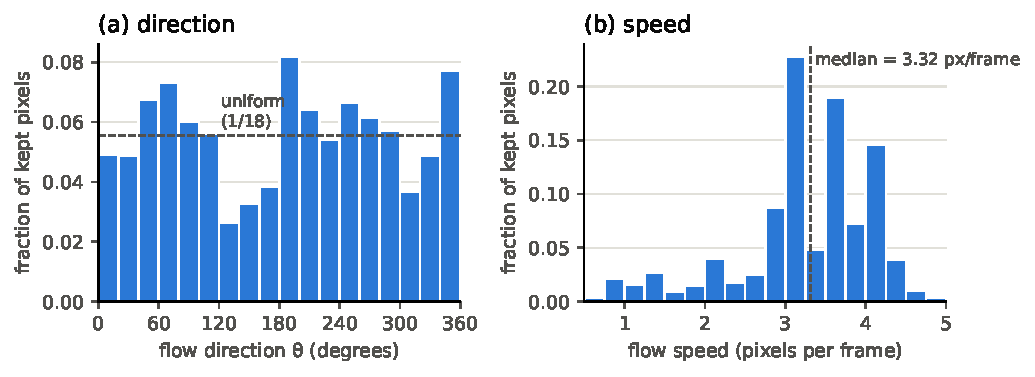
\includegraphics[width=0.9\textwidth]{fig1_flow.pdf}
\caption{Optical flow on the first 50 training videos (950 consecutive-frame pairs, Farneback).
Pixels kept: \FLOWNKEPT{} (above 0.2 intensity in both frames and flow magnitude above 0.5\,px).
(a) Flow direction, $\theta=\operatorname{atan2}(-d_y,d_x)$, as a fraction of kept pixels; the dashed line is
the uniform level $1/18$. (b) Flow speed; median \FLOWMEDIAN{}\,px/frame (dashed). Bars beyond 5\,px/frame
(0.46\% of kept pixels) are not drawn.}
\label{fig:1}
\end{figure}

\textbf{Q2.1.} \emph{Mirrored and rotated motion is already familiar.}
\begin{itemize}
\item Figure~1(a) has training motion in every direction and no empty sector. The bins vary between 0.026 and
0.082 around the uniform 0.056. That variation is what about 100 digit trajectories in 50 videos produce, not a
preferred direction.
\item Mirroring maps $\theta\mapsto180^\circ-\theta$, and a $90^\circ$ rotation maps
$\theta\mapsto\theta+90^\circ$. Applied to every training video, either would give a histogram that differs from
Figure~1(a) only by this sampling noise. So a model trained on these data has already seen mirrored and rotated
\emph{trajectories}, while mirrored and rotated \emph{digits} remain unfamiliar.
\end{itemize}

\emph{Faster motion is not.}
\begin{itemize}
\item Speeds are concentrated: median \FLOWMEDIAN{}\,px/frame, interquartile range 3.0--3.9, 90th percentile
4.1 (Figure~1(b)).
\item 2$\times$ and 3$\times$ correspond to about 6.6 and 10.0\,px/frame. Both lie outside what the training
data contain.
\end{itemize}

\emph{Overlap bias.} Where digits overlap, Farneback's single smooth flow field averages two motions. This
produces short or wrongly directed vectors, which feed the low-speed tail below 2\,px/frame or are dropped by the
0.5\,px threshold. Two $28\times28$ digits in a $64\times64$ frame overlap in only a minority of frames. The bias
can therefore blur the speed histogram's lower tail and add noise to direction bins, but it cannot fill or empty
a whole direction sector, nor move the 3--4\,px/frame peak. Neither conclusion changes.

\textbf{Q2.2.} Each transformation keeps the videos physically valid, because constant velocity with elastic
bounces in a square box is preserved:
\begin{itemize}
\item \textbf{Mirror} leaves the motion statistics essentially unchanged (Q2.1) and changes appearance: a
mirrored digit is not a digit.
\item \textbf{Rotation} likewise leaves the motion unchanged and changes appearance more: strokes swap orientation.
\item \textbf{Speed-up} leaves appearance unchanged (the same frames, subsampled) and changes only the motion,
pushing it outside the training range.
\end{itemize}
Each test therefore moves one factor while holding the other fixed. A failure under mirror or rotation points to
appearance; a failure under speed-up points to motion. Mirror and rotation give two doses of appearance change.
A model that has learned the motion rule itself should pass all three.

\subsection{Baseline: ConvLSTM}

\begin{table}[htbp]
\centering
\small
\caption{Test MSE per horizon, $E^{(5)}$ and trainable parameters at $1\times$, $t=1$; lower is better, entries are mean (seed 0, seed 1).}
\label{tab:2}
\resizebox{\textwidth}{!}{%
\begin{tabular}{lccccccc}
\toprule
Predictor & $\mathrm{MSE}_1$ & $\mathrm{MSE}_2$ & $\mathrm{MSE}_3$ & $\mathrm{MSE}_4$ & $\mathrm{MSE}_5$ & $E^{(5)}$ & Parameters \\
\midrule
Model A & 0.0168 (0.0170, 0.0167) & 0.0203 (0.0207, 0.0200) & 0.0226 (0.0230, 0.0221) & 0.0243 (0.0248, 0.0239) & 0.0259 (0.0264, 0.0255) & 0.0220 (0.0224, 0.0216) & 480{,}784 \\
Blank & 0.0426 & 0.0426 & 0.0426 & 0.0425 & 0.0425 & 0.0426 & 0 \\
Copy-last & 0.0492 & 0.0604 & 0.0669 & 0.0708 & 0.0732 & 0.0641 & 0 \\
\bottomrule
\end{tabular}}
\end{table}


\begin{figure}[H]
\centering
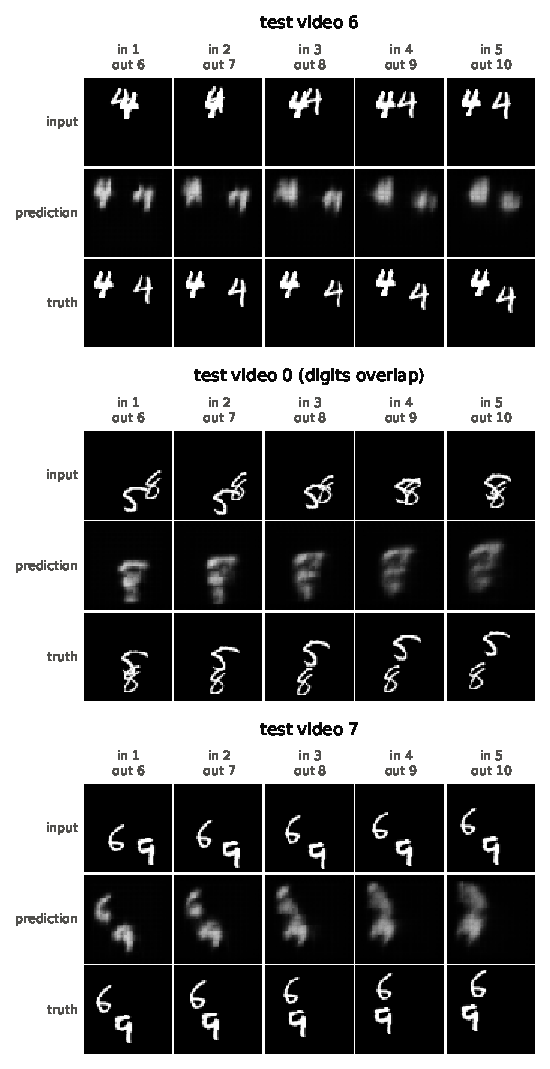
\includegraphics[width=0.56\textwidth]{fig2_examples.pdf}
\caption{Model A (seed 0) on three test videos at 1$\times$, $t=1$. In each block: the input frames 1--5, the
prediction and the ground truth for frames 6--10. Test video 0 (dataset index 9000) has overlapping digits;
videos 6 and 7 (9006, 9007) do not.}
\label{fig:2}
\end{figure}

\textbf{Q2.3.} Model A's reach is \textbf{8 pixels per time step} (2 cells of the folded grid).
\begin{itemize}
\item \emph{Folding.} \texttt{pixel\_unshuffle(4)} regroups each $4\times4$ patch into 16 channels, so one cell
of the $16\times16$ grid is 4\,px. It moves no information, and neither do the $1\times1$ head and
\texttt{pixel\_shuffle}.
\item \emph{One step $\tau$ has exactly two spatial operations:} layer~1's $3\times3$ convolution on
$[u_\tau,h^{(1)}_{\tau-1}]$ and layer~2's $3\times3$ convolution on $[h^{(1)}_\tau,h^{(2)}_{\tau-1}]$. Each moves
information at most one cell. The gates and the cell-state update (Eq.~4) are element-wise, so $c$ moves nothing.
\item \emph{Paths to $\hat x_{\tau+1}$.}
  \begin{itemize}
  \item From the new input: $u_\tau\to$ conv\textsubscript{1} $\to$ conv\textsubscript{2}, 2 cells.
  \item From layer~1's state: $h^{(1)}_{\tau-1}\to$ conv\textsubscript{1} $\to$ conv\textsubscript{2}, 2 cells.
  \item From layer~2's state: $h^{(2)}_{\tau-1}\to$ conv\textsubscript{2}, 1 cell.
  \item From layer~1's cell state: $c^{(1)}_{\tau-1}\to h^{(1)}_\tau\to$ conv\textsubscript{2}, 1 cell.
  \end{itemize}
  The longest is 2 cells, i.e.\ $2\times4=8$\,px along each axis. Because $3\times3$ kernels include diagonal
  neighbours, it is up to $8\sqrt2\approx11.3$\,px diagonally.
\item \emph{Recurrence.} The recurrence does not extend this. Information can travel further over several steps,
but tracking needs the digit's new position in $u_\tau$ to meet its old position, held in $h_{\tau-1}$, within
one update. During the rollout the fed-back prediction plays the role of $u_\tau$, so the same limit applies.
\end{itemize}

\textbf{Q2.4.}
\begin{itemize}
\item \emph{Against the references.} Model A's $E^{(5)}=0.0220$ is about half of Blank's (0.0426) and a third
of Copy-last's (0.0641), and the two seeds agree closely (0.0224, 0.0216). Copy-last is worse than Blank because
a stationary copy is wrong twice: it leaves ink where the digits were and none where they are now.
\item \emph{Growth over the horizons.} Model A's error rises from $\mathrm{MSE}_1=0.0168$ to
$\mathrm{MSE}_5=0.0259$ ($+54\%$). The first step costs most ($+21\%$); after that the increments shrink ($+11\%$, $+8\%$,
$+7\%$), while Blank's error stays flat. Figure~2 shows where the error comes from: positions stay roughly right, but every
step loses detail, and by $h=5$ the digits are blobs. Blurring is what a squared-error forecaster does under
uncertainty, because it averages over plausible futures instead of committing to one sharp, possibly wrong, frame.
\item \emph{Overlap.} In test video~0 the 5 and the 8 overlap in the inputs, and model A predicts one merged
smear that drifts with their average motion. When the true digits separate (the 5 up and right, the 8 down and
left), the prediction does not split. It stretches along the line between them. Test video~7 shows the same
merging as the 6 and the 9 approach each other. The ConvLSTM keeps no separate object identities: two digits on
the same cells share the same state, so once they overlap their shapes and velocities mix and cannot be recovered.
\end{itemize}

\textbf{Q2.5} (recorded before any Testing-the-Baseline experiment; reproduced unchanged from
\texttt{report/prerun\_predictions.md}).
Approved by the student and committed at 2026-10-27 15:23 PKT (commit \texttt{33d4a9f}), before any of the
experiments below.

\begin{quote}\small
\textbf{Mirror test: should pass, approximately.}
Figure 1(a) shows training motion in every direction with no empty sector, so a mirrored trajectory
($\theta\to180^\circ-\theta$) is familiar motion. Only the digits look unfamiliar.
Model A is convolutional and mostly has to carry local strokes along, so mirrored digits should cost little.
Expected: $E_M$ within about 10\% of $E^{(5)}$, and $C_M$ well below $E_M$.

\textbf{Rotation test: should also pass, but less cleanly than mirror.}
A $90^\circ$ rotation ($\theta\to\theta+90^\circ$) again gives familiar motion. But it turns vertical strokes into
horizontal ones, and the learned $3\times3$ filters are not rotation-equivariant, so the appearance shift is larger.
Expected: $E_R>E_M$ and $C_R>C_M$, with $E_R$ up to about 20--30\% above $E^{(5)}$. Degraded, not broken.

\textbf{Speed-up: should break down at 3$\times$.}
Model A's reach is 8\,px per time step along each axis (Q2.3; up to $8\sqrt2\approx11.3$\,px diagonally). The
median training speed is 3.3\,px/frame (Figure 1(b)), so 2$\times\approx$ 6.6\,px/frame and 3$\times\approx$
10\,px/frame.
At 2$\times$, motion stays within reach but is faster than anything in training (90th percentile 4.1\,px/frame).
Predictions should degrade, with digits lagging behind their true positions, but stay roughly on track.
At 3$\times$, the displacement exceeds the reach for most directions (any motion within about $37^\circ$ of an
axis). The network cannot link a digit's old position to its new one in one update. Digits should lag, smear or
fade, and $E^{(2)}$ should come close to, or exceed, Copy-last's.
\end{quote}

\subsection{Testing the Baseline}

\textbf{Mirror and rotation.}

\begin{table}[htbp]
\centering
\small
\caption{Test error and consistency under mirror ($M$) and rotation ($R$) at $1\times$; lower is better, entries are mean (seed 0, seed 1).}
\label{tab:3}
\resizebox{\textwidth}{!}{%
\begin{tabular}{lccccc}
\toprule
Predictor & $E^{(5)}$ & $C_M$ & $E_M$ & $C_R$ & $E_R$ \\
\midrule
Model A & 0.0220 (0.0224, 0.0216) & 0.00186 (0.00179, 0.00194) & 0.0226 (0.0231, 0.0222) & 0.00312 (0.00315, 0.00309) & 0.0238 (0.0241, 0.0235) \\
Blank & 0.0426 & 0 & 0.0426 & 0 & 0.0426 \\
Copy-last & 0.0641 & 0 & 0.0641 & 0 & 0.0641 \\
\bottomrule
\end{tabular}}
\end{table}


\begin{figure}[H]
\centering
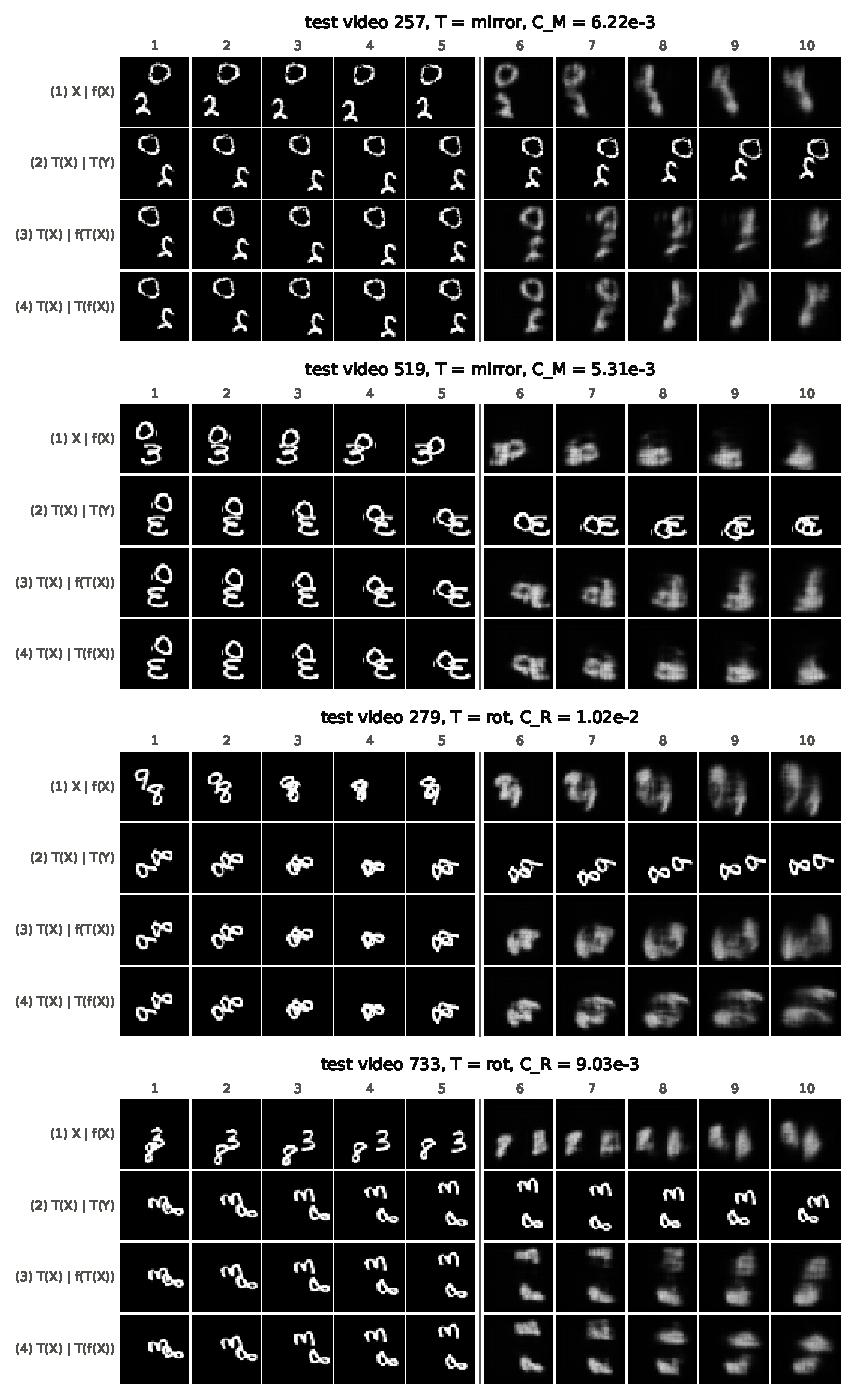
\includegraphics[width=0.84\textwidth]{fig3_consistency.pdf}
\caption{The two test videos with the largest per-video $C_M$ (top two panels, $T$ = mirror) and $C_R$ (bottom
two, $T$ = $90^\circ$ rotation) for seed-0 model A. Columns 1--5 are the inputs, columns 6--10 the five forecast
horizons. Rows: (1) $X\mid f(X)$, (2) $T(X)\mid T(Y)$, (3) $T(X)\mid f(T(X))$, (4) $T(X)\mid T(f(X))$. Rows 3
and 4 should agree for a consistent model. GIFs stepping through the horizons with the same four rows:
\texttt{Question2/results/gifs/fig3\_mirror\_257.gif}, \texttt{fig3\_mirror\_519.gif},
\texttt{fig3\_rot\_279.gif}, \texttt{fig3\_rot\_733.gif}.}
\label{fig:3}
\end{figure}

\begin{figure}[H]
\centering
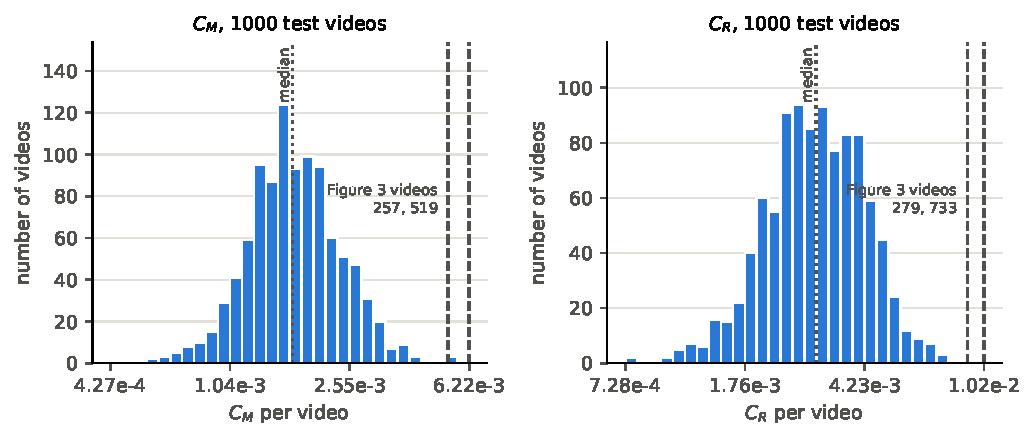
\includegraphics[width=0.9\textwidth]{fig4_hist.pdf}
\caption{Per-video consistency gaps of seed-0 model A over the 1,000 test videos (log-spaced bins). Dotted line:
the median. Dashed lines: the Figure~3 videos.}
\label{fig:4}
\end{figure}

\textbf{Q2.6.} Blank and Copy-last commute with every pixel rearrangement. The zero frame stays zero, and copying
the last frame and then transforming gives the same result as transforming and then copying. So $C_M=C_R=0$
exactly, yet their transformed errors (0.0426 and 0.0641) are two to three times model A's. A forecaster that
ignores the motion altogether is perfectly consistent: $C_T$ only says whether the model treats a transformed
scene the \emph{same way}, not whether it treats it \emph{correctly}. $E_T$ measures the second, so a small $C_T$
is only good news next to a small $E_T$. Model A has both: $C_M=1.86\times10^{-3}$ is about 8\% of $E_M=0.0226$.

\textbf{Q2.7.} Test video 257 under mirroring ($C_M=6.22\times10^{-3}$, the largest).
\begin{itemize}
\item \emph{The truth} (row 2): the 0 stays near the top right, while the mirrored 2 climbs up and to the right
towards it.
\item \emph{Row 4} (the upright forecast, mirrored afterwards) keeps that account. The 2 moves up towards the 0,
and by frame 10 the two have merged into one leaning, forked streak near the true position.
\item \emph{Row 3} (the forecast from the mirrored input) loses the 2. It fades after frame 7, and the 0 melts into
a single vertical bar below and to the left of where the digits actually go.
\end{itemize}
Shown the same motion with mirrored digits, the model no longer moves the 2 at all: one digit gets lost, and the
other blurs into an unrecognisable stroke that drifts the wrong way. All four Figure~3 videos have digits that
overlap or close in on each other, where the shapes are needed to tell the two digits apart.

\textbf{Q2.8.} Yes, rotation is harder:
\begin{itemize}
\item $C_R=3.12\times10^{-3}$ is 1.7 times $C_M=1.86\times10^{-3}$.
\item $E_R$ is 8\% above $E^{(5)}$, against 3\% for $E_M$.
\item Both seeds agree, and Figure~4 shows that the whole $C_R$ distribution is shifted to the right, not just its
tail.
\end{itemize}
The motion cannot explain the difference. By Q2.1 both transformations give equally familiar motion, because the
training directions cover the circle evenly and speeds are unchanged. By Q2.2, what separates them is how much they
change the digits' appearance. A mirror keeps vertical strokes vertical and horizontal strokes horizontal; a
$90^\circ$ rotation swaps them, so rotated digits are further from anything the filters were trained on. The gap
therefore comes from appearance. It is largest where two digits overlap and the model has to rely on their shapes
to keep them apart.

\textbf{Faster motion.}

\begin{table}[htbp]
\centering
\small
\caption{Test error of model A at speeds $1\times,2\times,3\times$ (start $t=1$); lower is better, entries are mean (seed 0, seed 1).}
\label{tab:4}
\resizebox{\textwidth}{!}{%
\begin{tabular}{lccccc}
\toprule
Predictor & $E^{(2)}$ $1\times$ & $E^{(2)}$ $2\times$ & $E^{(2)}$ $3\times$ & $E^{(5)}$ $1\times$ & $E^{(5)}$ $2\times$ \\
\midrule
Model A & 0.0186 (0.0188, 0.0184) & 0.0461 (0.0461, 0.0461) & 0.0540 (0.0537, 0.0543) & 0.0220 (0.0224, 0.0216) & 0.0515 (0.0509, 0.0522) \\
Copy-last & 0.0548 & 0.0661 & 0.0703 & 0.0641 & 0.0719 \\
\bottomrule
\end{tabular}}
\end{table}


\begin{figure}[H]
\centering
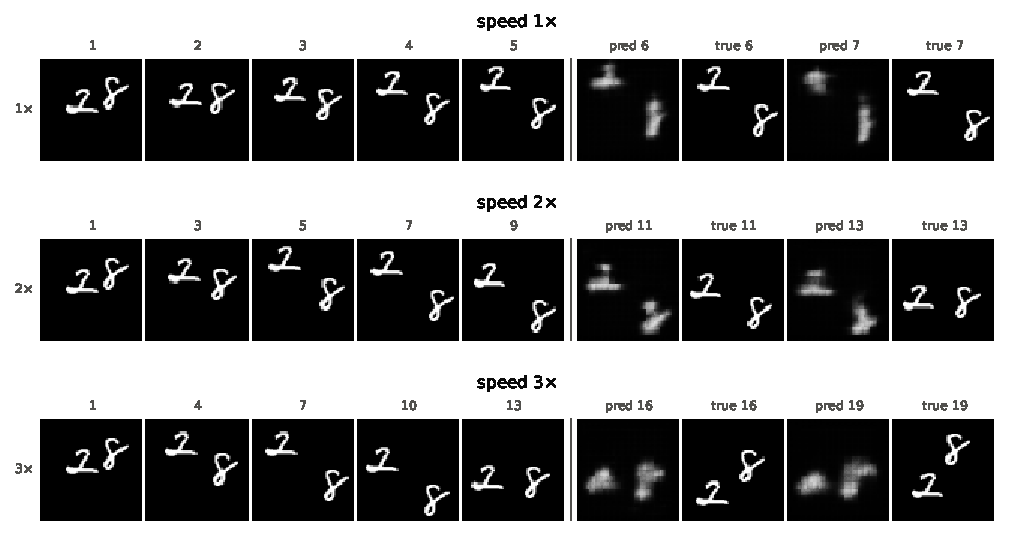
\includegraphics[width=0.9\textwidth]{fig5_speeds.pdf}
\caption{Seed-0 model A on test video 29 at $1\times$, $2\times$ and $3\times$ ($t=1$): the five input frames,
then the first two predicted and true future frames. The digits do not overlap in any displayed true frame.}
\label{fig:5}
\end{figure}

\textbf{Q2.9.} Model A's predictions fall apart at \textbf{2$\times$}:
\begin{itemize}
\item $E^{(2)}$ rises from 0.0186 at 1$\times$ to 0.0461 at 2$\times$ (2.5 times), already worse than predicting
an empty frame (Blank: 0.0426).
\item At 3$\times$ it reaches 0.0540. It stays below Copy-last (0.0661 and 0.0703) only because a blurred guess
costs less than a sharp digit in the wrong place.
\end{itemize}
This only partly agrees with the reach estimate. The 3$\times$ failure fits, because about 10\,px/frame exceeds
the 8\,px reach for most directions. The 2$\times$ failure does not, because about 6.6\,px/frame is within reach.
The estimate missed that reach is necessary but not sufficient. It counts the longest path that \emph{could} carry
information, but the network only learned to use the displacements it was trained on (3--4\,px/frame), and the
contribution from the edge of the $5\times5$-cell window is weak.

Figure~5 shows what happens instead: \emph{stalling}. At 2$\times$, the predicted 2 and 8 stay near their positions
in the last input frame (9), while the true 2 moves on and the true 8 bounces upwards. At 3$\times$, both digits
sit where they were in frame 13 and fade into blobs. There are no duplicated or wrongly moving digits. The model
cannot link the new positions to the old ones, so it keeps the mass where it last saw it and blurs it to hedge.
This is the behaviour of a model that has not found the motion, rather than one that applies the wrong motion.

\textbf{Q2.10.} No. For model A the two explanations coincide: both 2$\times$ and 3$\times$ are faster than
anything in training, and 3$\times$ is also beyond reach. The 2$\times$ failure shows that unfamiliar motion
\emph{alone} can break the model, which makes it impossible to decide from these runs whether reach also matters
at 3$\times$. The separating experiment keeps the architecture and changes only the data:
\begin{itemize}
\item Train the same network with speed augmentation ($k\sim U\{1,2,3\}$), i.e.\ model C.
\item If C fixes 2$\times$ but still fails at 3$\times$, the 3$\times$ failure is architectural reach.
\item If C also fixes 3$\times$, the failure was unfamiliar motion.
\item The complementary control is a model with larger reach trained on the same speed-augmented data (model D):
it should succeed at 3$\times$ exactly where C fails, if reach is the limit.
\end{itemize}

\subsection{What Can Data Fix?}
\textbf{Q2.11} (approved by the student and committed and pushed at 2026-10-27 15:34 PKT, commit
\texttt{eeee372}, before any of models B--D or any D candidate was trained; reproduced unchanged).

\begin{quote}\small
Model B should fix the mirror and rotation failures ($C_M$ and $C_R$ several times smaller, and $E_M$ and $E_R$
close to its own $E^{(5)}$), because those failures come from unfamiliar appearance, but it should do nothing for
speed. Model C should fix 2$\times$, which is unfamiliar motion still within model A's 8-px reach, but keep failing
at 3$\times$ (about 10\,px/frame, beyond that reach for most directions), however much fast motion it sees in
training. Only model D, with a larger reach and the same speed augmentation, should also handle 3$\times$; each of
B, C and D may give up a little accuracy at 1$\times$.
\end{quote}

\textbf{Choosing model D (validation split only).}
\begin{itemize}
\item Three candidates were compared. Each has a one-step reach of 16\,px and at most 721,176 parameters.
  \begin{itemize}
  \item \emph{dil}: layer~2's $3\times3$ convolution dilated by 3; 480,784 parameters.
  \item \emph{k5}: $5\times5$ kernels with 46 hidden channels; 709,520.
  \item \emph{p8}: $8\times8$ folding; 594,496.
  \end{itemize}
\item Each was trained once (seed 0) under model D's protocol and scored on the 1,000 validation videos. The rule,
fixed before any candidate was trained: lowest mean validation $E^{(2)}$ over 1$\times$, 2$\times$ and 3$\times$.
\item \emph{p8} won (0.0302; \emph{dil} 0.0308). In its single run, \emph{k5} collapsed to an almost constant
output (0.0395 at every speed); it was not tuned further.
\item The full screen is in \texttt{Question2/results/metrics/d\_screening.json} (\texttt{screen\_d.py}).
\end{itemize}

\begin{table}[htbp]
\centering
\small
\caption{Test results for models A--D (rows: quantities; columns: models); lower is better for all rows, entries are mean (seed 0, seed 1). $E^{(2)}$ is used across speeds, with $t=1$.}
\label{tab:5}
\resizebox{\textwidth}{!}{%
\begin{tabular}{lcccc}
\toprule
Quantity & A & B & C & D \\
\midrule
$E^{(5)}$ $1\times$ & 0.0220 (0.0224, 0.0216) & 0.0223 (0.0233, 0.0214) & 0.0278 (0.0278, 0.0277) & 0.0296 (0.0306, 0.0286) \\
\midrule
$C_M$ & 0.00186 (0.00179, 0.00194) & 0.00116 (0.00106, 0.00126) & 0.00102 ($8.76\times10^{-4}$, 0.00116) & 0.00122 ($6.06\times10^{-4}$, 0.00183) \\
$E_M$ & 0.0226 (0.0231, 0.0222) & 0.0224 (0.0233, 0.0215) & 0.0280 (0.0280, 0.0280) & 0.0298 (0.0307, 0.0288) \\
$C_R$ & 0.00312 (0.00315, 0.00309) & 0.00143 (0.00134, 0.00151) & 0.00197 (0.00180, 0.00214) & 0.00179 (0.00117, 0.00242) \\
$E_R$ & 0.0238 (0.0241, 0.0235) & 0.0223 (0.0232, 0.0215) & 0.0287 (0.0287, 0.0288) & 0.0303 (0.0312, 0.0295) \\
\midrule
$E^{(2)}$ $1\times$ & 0.0186 (0.0188, 0.0184) & 0.0188 (0.0195, 0.0181) & 0.0238 (0.0241, 0.0236) & 0.0276 (0.0285, 0.0267) \\
$E^{(2)}$ $2\times$ & 0.0461 (0.0461, 0.0461) & 0.0439 (0.0437, 0.0441) & 0.0294 (0.0296, 0.0293) & 0.0295 (0.0303, 0.0286) \\
$E^{(2)}$ $3\times$ & 0.0540 (0.0537, 0.0543) & 0.0491 (0.0490, 0.0492) & 0.0337 (0.0337, 0.0338) & 0.0319 (0.0330, 0.0308) \\
\midrule
Trainable parameters & 480{,}784 & 480{,}784 & 480{,}784 & 594{,}496 \\
\midrule
Training time per epoch (s) & 6.39 (6.39, 6.40) & 6.52 (6.53, 6.52) & 6.42 (6.43, 6.41) & 2.39 (2.38, 2.39) \\
Inference time (s) & 0.235 (0.236, 0.235) & 0.243 (0.242, 0.244) & 0.243 (0.242, 0.243) & 0.0813 (0.0811, 0.0815) \\
\bottomrule
\end{tabular}}
\end{table}


\textbf{Q2.12.} Model D is model A with $8\times8$ instead of $4\times4$ folding.
\begin{itemize}
\item \texttt{pixel\_unshuffle(x, 8)} turns a $1\times64\times64$ frame into $64\times8\times8$.
\item Two ConvLSTM layers follow (64 hidden channels, $3\times3$ kernels).
\item A $1\times1$ convolution maps 64 to 64 channels, then \texttt{pixel\_shuffle}$(\cdot,8)$ and a sigmoid.
\item 594,496 parameters, below the 721,176 cap. Everything else (shapes, 9-step rollout without teacher forcing,
training protocol) is identical to model A.
\end{itemize}
Its reach follows the same argument as Q2.3. One step has two spatial operations, the $3\times3$ convolutions of
layers~1 and~2, each moving information one cell. The longest path ($u_\tau$ or $h^{(1)}_{\tau-1}$ through both
convolutions) therefore crosses 2 cells, but a cell is now 8\,px wide. Reach $=2\times8=$ \textbf{16\,px} per
axis ($16\sqrt2\approx22.6$\,px diagonally), \textbf{twice model A's 8\,px}, so strictly larger. At 3$\times$ the
median displacement is about 10\,px/frame and the 90th percentile about 12.4\,px/frame, inside D's reach in every
direction. Coarser folding is the price: each output cell must rebuild an $8\times8$ patch from 64 hidden channels.


\textbf{Q2.13.}
\begin{itemize}
\item \emph{Mirror and rotation (Table~3): appearance.}
  \begin{itemize}
  \item Model B changes only the training appearance (no new speeds). It cuts $C_M$ from $1.86\times10^{-3}$ to
  $1.16\times10^{-3}$ and $C_R$ from $3.12\times10^{-3}$ to $1.43\times10^{-3}$, and closes the rotation error gap
  completely: $E_R=0.0223$ equals B's own $E^{(5)}$, against $+8\%$ for A.
  \item Models C and D, trained without symmetry augmentation, keep $E_R$ above $E^{(5)}$ ($+3.5\%$, $+2.5\%$).
  Their smaller $C_T$ comes with a much larger $E_T$: blurrier forecasts are more consistent for free (Q2.6).
  \end{itemize}
\item \emph{2$\times$: unfamiliar motion.} Model C has exactly A's architecture and reach, only trained on faster
clips. It cuts $E^{(2)}$ at 2$\times$ from 0.0461 to 0.0294 ($-36\%$). B, which sees no new speeds, barely moves it
(0.0439).
\item \emph{3$\times$: mostly unfamiliar motion, with a smaller reach component.}
  \begin{itemize}
  \item C, with A's 8\,px reach, already cuts $E^{(2)}$ at 3$\times$ from 0.0540 to 0.0337 ($-38\%$).
  \item D, with twice the reach, lowers it further to 0.0319.
  \item The clearer reach signal is the slope: from 1$\times$ to 3$\times$, C's error rises by 42\% and D's by
  only 16\%.
  \end{itemize}
\end{itemize}

So model C does \emph{not} do badly at 3$\times$. Reach was not the binding limit for most of the motion, for two
reasons. First, a digit is about 20\,px wide, so after a 10\,px jump its new position still overlaps its old one
within 8\,px, and the network can link the two through that overlap. Second, diagonal motion stays inside the
$8\sqrt2\approx11.3$\,px diagonal reach. Had C failed where D succeeded, it would have shown that the information
simply cannot reach the right place in one update. More data could never fix that. Training changes the weights on
the paths the convolutions provide, not the paths themselves: no setting of the weights can make an output cell
depend on an input cell outside its receptive field. Data can only teach the network to use the reach it has.

\textbf{Q2.14.} Yes, for the speed-augmented models.
\begin{itemize}
\item \emph{B.} No cost: its $E^{(5)}$ at 1$\times$ is 0.0223 against A's 0.0220, inside the seed spread.
Seed~1 of B (0.0214) even beats both A seeds.
\item \emph{C.} $+26\%$ (0.0278). It spends two-thirds of its windows on other speeds within the same 30 epochs,
and its training loss is still well above A's at the end (Figure~S1).
\item \emph{D.} $+35\%$ (0.0296). Two causes: the coarser $8\times8$ folding blurs detail (Figure~6(b) shows
blocky forecasts), and the optimisation stalls. Every $8\times8$-folding run sits on a near-blank plateau
(training loss $\approx0.040$) for 10--20 epochs before it starts learning (Figure~S1), so D is under-trained
relative to A and C under the fixed budget.
\end{itemize}
Was it worth it? For a forecaster meant to model motion, yes. C and D lower $E^{(2)}$ by 36\% at 2$\times$ and by
38--41\% at 3$\times$, and their worst-speed errors (0.0337 and 0.0319) are far below A's (0.0540). That is a
gain of 0.017 at 2$\times$ and 0.020--0.022 at 3$\times$, against a 1$\times$ loss of 0.006--0.008. For a service that only ever sees 1$\times$ clips, it is
not: symmetrised B is the most accurate model at 1$\times$.

\begin{figure}[H]
\centering
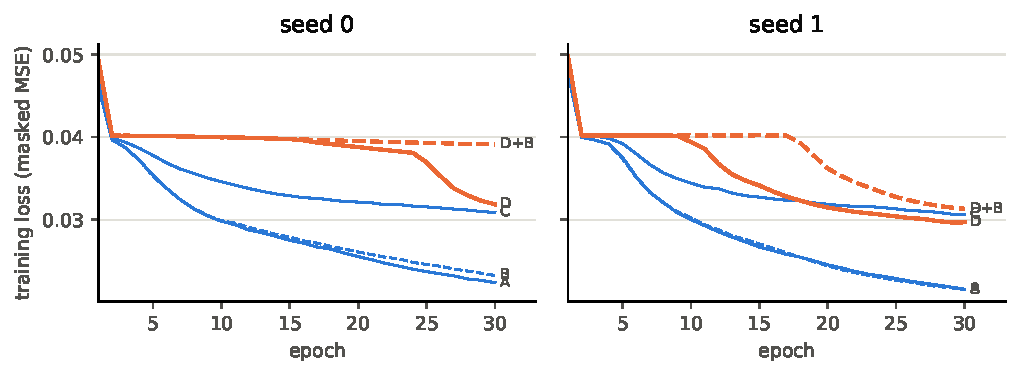
\includegraphics[width=0.9\textwidth]{figS1_loss.pdf}
\caption*{\textbf{Figure S1} (supplementary). Training loss per epoch for every learned model and seed (blue:
$4\times4$ folding, A--C; orange: $8\times8$ folding, D and D+B; dashed: with symmetry augmentation). The
$8\times8$-folding runs sit on a plateau near 0.040 (an almost constant forecast) before they start to learn; D+B
seed~0 never leaves it within the 30 epochs.}
\end{figure}

\subsection{The Final Model}
\textbf{Exact symmetry of $\bar f$.} Take any $T\in G$. Because $G$ is a group, $g'=gT$ runs over all of $G$
when $g$ does, and $g^{-1}=T\,g'^{-1}$. Hence
\[
\bar f(TX)=\tfrac18\sum_{g\in G}g^{-1}f(gTX)=\tfrac18\sum_{g'\in G}T\,g'^{-1}f(g'X)=T\Big(\tfrac18\sum_{g'}g'^{-1}f(g'X)\Big)=T\bar f(X),
\]
using that $T$ is linear (a pixel permutation). This holds for every input and any $f$, so $C_M=C_R=0$ exactly.
The measured values ($\sim10^{-17}$, Table~6) are float32 rounding from summing the same eight terms in a different
order. Because MSE is unchanged when the same permutation is applied to both arguments, it also follows that
$E_M=E_R=E^{(5)}$ for every symmetrised model.

\textbf{Which final model.} We first chose D+B, before evaluating it, on the strength of Table~5: model~B shows that
symmetry augmentation costs nothing at 1$\times$ and makes transformed inputs as accurate as the originals, which
is exactly what the symmetrised forecaster averages over. The D+B seed~0 run, however, never left the $8\times8$
plateau within the 30 epochs: its training loss was 0.0391 at the end (Figure~S1), and its forecasts are almost
constant ($E^{(5)}=0.0390$ at every horizon and speed). The protocol fixes the seeds and the number of epochs, so
it cannot be rerun. A final model with one failed seed out of two is not reliable, so \textbf{the final model is
symmetrised D}. For reference, symmetrised D+B gives $E^{(5)}=0.0300$ for seed~1 and 0.0390 for seed~0.

\begin{table}[htbp]
\centering
\small
\caption{Test results for symmetrised models (rows: quantities; columns: models); lower is better, entries are mean (seed 0, seed 1). Training time is that of the underlying learned model.}
\label{tab:6}
\resizebox{\textwidth}{!}{%
\begin{tabular}{lcc}
\toprule
Quantity & Sym.\ B & Sym.\ D \\
\midrule
$E^{(5)}$ $1\times$ & 0.0218 (0.0227, 0.0208) & 0.0294 (0.0305, 0.0283) \\
\midrule
$C_M$ & $8.63\times10^{-17}$ ($8.55\times10^{-17}$, $8.71\times10^{-17}$) & $6.17\times10^{-17}$ ($5.82\times10^{-17}$, $6.52\times10^{-17}$) \\
$E_M$ & 0.0218 (0.0227, 0.0208) & 0.0294 (0.0305, 0.0283) \\
$C_R$ & $6.97\times10^{-17}$ ($6.94\times10^{-17}$, $7.01\times10^{-17}$) & $4.78\times10^{-17}$ ($4.63\times10^{-17}$, $4.92\times10^{-17}$) \\
$E_R$ & 0.0218 (0.0227, 0.0208) & 0.0294 (0.0305, 0.0283) \\
\midrule
$E^{(2)}$ $1\times$ & 0.0184 (0.0191, 0.0176) & 0.0275 (0.0285, 0.0265) \\
$E^{(2)}$ $2\times$ & 0.0431 (0.0430, 0.0432) & 0.0292 (0.0302, 0.0283) \\
$E^{(2)}$ $3\times$ & 0.0482 (0.0481, 0.0482) & 0.0317 (0.0329, 0.0305) \\
\midrule
Trainable parameters & 480{,}784 & 594{,}496 \\
\midrule
Training time per epoch (s) & 6.52 (6.53, 6.52) & 2.39 (2.38, 2.39) \\
Inference time (s) & 2.71 (2.71, 2.71) & 0.549 (0.550, 0.549) \\
\bottomrule
\end{tabular}}
\end{table}


\begin{figure}[p]
\centering
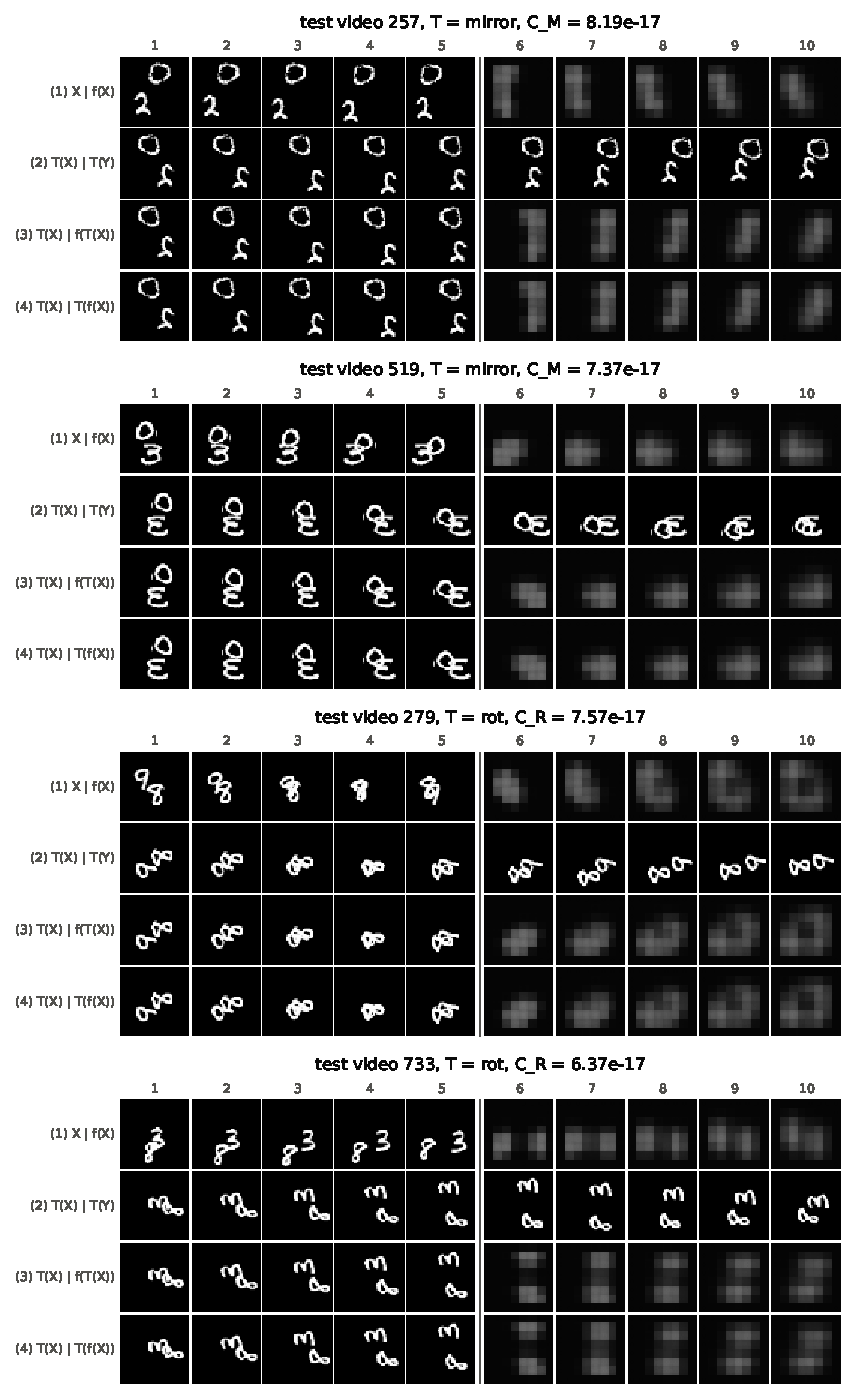
\includegraphics[width=0.55\textwidth]{fig6a_consistency.pdf}\\[2pt]
\textbf{(a)}\\[4pt]
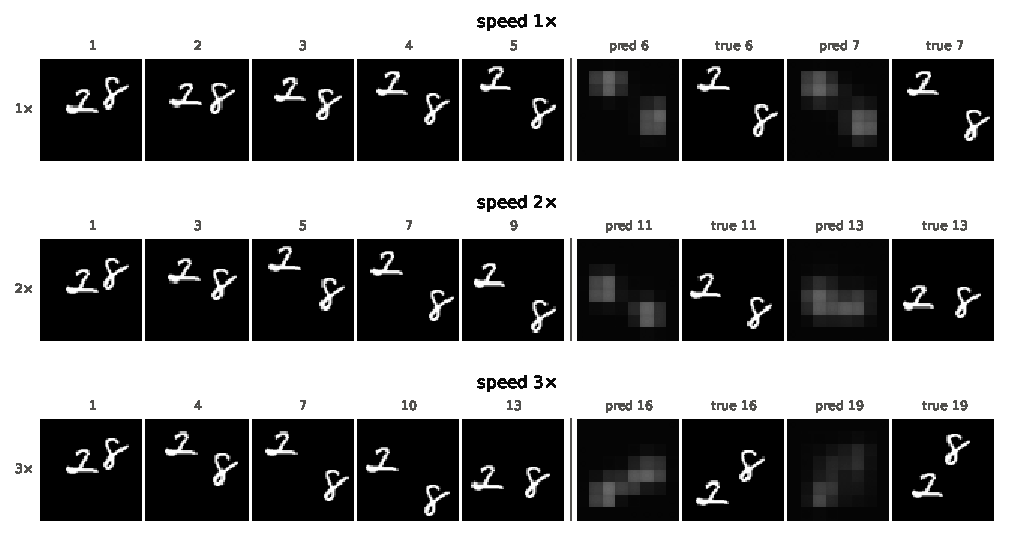
\includegraphics[width=0.78\textwidth]{fig6a_speeds.pdf}\\
\textbf{(b)}
\caption{The final model (symmetrised D, seed 0). (a) Figure~3 repeated on the same videos and transformations;
rows 3 and 4 now coincide. GIFs: \texttt{Question2/results/gifs/fig6a\_mirror\_257.gif},
\texttt{fig6a\_mirror\_519.gif}, \texttt{fig6a\_rot\_279.gif}, \texttt{fig6a\_rot\_733.gif}. (b) Figure~5
repeated on test video 29.}
\label{fig:6}
\end{figure}

\textbf{Q2.15.}
\begin{itemize}
\item \emph{Consistency.} Learned symmetry (B) reduces the gaps but does not remove them:
$C_M=1.16\times10^{-3}$ and $C_R=1.43\times10^{-3}$. Built-in symmetry gives $\sim10^{-17}$. Only the built-in
version is exact, because the proof above holds for every input and every $f$. Augmentation only rewards
consistency on the training distribution, on average, through the loss.
\item \emph{Accuracy on original clips.} Symmetrised B is slightly better than B ($E^{(5)}$ 0.0218 against
0.0223), and symmetrised D matches D (0.0294 against 0.0296).
\item \emph{Accuracy on transformed clips.} The built-in models have $E_M=E_R=E^{(5)}$ by construction (0.0218
for symmetrised B), against B's 0.0224 and 0.0223.
\item \emph{Inference cost.} Eight forward passes plus transforms. Symmetrised B takes 2.71\,s for the 1,000 test
videos against B's 0.243\,s (11$\times$); symmetrised D takes 0.549\,s against 0.081\,s (6.8$\times$).
\end{itemize}

\emph{When averaging hurts.} Squared error is convex, so the averaged forecast can never be worse than the
\emph{average} of the eight back-transformed forecasts' errors. It hurts when some of those eight are much worse
than the untransformed one, because averaging then blurs a sharp, good forecast with poor ones. This happens when
the model has not learned the transformed inputs, or when the data are not truly symmetric (gravity, text,
lighting from above). Here the data are symmetric and the eight forecasts are similar, so averaging acted like a
small ensemble and did not hurt: $E^{(5)}$ fell by 2.6\% for B and by 0.8\% for D.

\textbf{Q2.16.} Test video 257, mirrored (Figure~6(a), top panel).
\begin{itemize}
\item \emph{Fixed by symmetrisation.} Rows 3 and 4 are now identical ($C_M=8.19\times10^{-17}$). The final model no
longer has one account of the motion for the upright video and another for the mirrored one: the 2 is not dropped
on the mirrored input any more.
\item \emph{Not fixed.} The forecast is still not right. Both digits become one blocky column of $8\times8$ cells,
which leans and drifts up and to the right, roughly following the 2 as it climbs towards the 0. Neither digit
stays recognisable, and they do not stay apart. Symmetrisation removed the inconsistency, and the speed
augmentation and larger reach do not matter at 1$\times$. The coarser $8\times8$ folding made the shapes worse,
not better.
\end{itemize}

\textbf{Q2.17 (final verdict).} Partly. The final model has learned where moving mass goes, but not what moves. It
is exactly consistent under mirror and rotation, and its error barely depends on speed: $E^{(2)}$ rises by 15\% from
1$\times$ to 3$\times$, against 190\% for model A. Figure~6(b) shows it sending both digits in the right directions
at 3$\times$, where A stalled. What would convince a skeptic is success on motion it never saw: intermediate or
higher speeds within its 16\,px reach (1.5$\times$, 4$\times$), and new shapes such as letters, with errors close
to those at 1$\times$. One test it still fails: keeping two digits apart after they overlap (Figure~6(a)). Its
forecasts merge them into one blocky blob, and its 1$\times$ accuracy (0.0294) is worse than model A's (0.0220).

\clearpage
\appendix
\section{Use of generative AI}

Tool: Claude (Anthropic) via Claude Code, used throughout as a coding, analysis and writing
assistant; it wrote and executed code in the student's environment and drafted report text.
In line with the course AI policy, each row gives the prompt (paraphrased in formal language,
preserving its substance), what the tool produced, and what the student changed or decided.
Every number in this report is produced by, and reproducible from, the code in the repository.

{\footnotesize
\begin{longtable}{p{0.025\textwidth}p{0.11\textwidth}p{0.26\textwidth}p{0.26\textwidth}p{0.21\textwidth}}
\toprule
\# & Stage & Prompt (paraphrased) & Output & Student edits and decisions \\ \midrule
\endhead
1 & Planning & Read the assignment handout and its front-page instructions. Without writing code or installing anything, assess whether both questions can be completed, and propose an approach that keeps accuracy while limiting cost, delegating sub-tasks to lower-cost models. & A feasibility analysis for Question 1 (written design) and Question 2 (experiment pipeline checked against the handout's built-in checks). A diagnosis of why the local GPU driver failed to load. A staged plan with a model allocation per sub-task, and a list of decisions for the student. & Reported the deadline extension to Oct 29. Fixed the GPU driver personally by enrolling the Secure Boot key. Chose to manage all GitHub commits and pushes personally. Asked for the Q2.5 and Q2.11 predictions to be drafted by the tool and reviewed by the student before they are recorded. \\ \midrule
2 & Environment & Set up the environment before any experiment, following the approach used in Assignment 1. & A Python 3.12 virtual environment reusing the existing CUDA build of PyTorch 2.9.0, with the matching torchvision 0.24.0, OpenCV, matplotlib and imageio. The Moving MNIST download. A repository skeleton (report folder, this log, the pre-run predictions file). & None. \\ \midrule
\bottomrule
\end{longtable}
}


\section*{References}
\small
\begin{itemize}[leftmargin=*]
\item X.~Shi, Z.~Chen, H.~Wang, D.-Y.~Yeung, W.-K.~Wong, W.~Woo. Convolutional LSTM Network: A Machine
Learning Approach for Precipitation Nowcasting. \textit{NeurIPS}, 2015.
\item N.~Srivastava, E.~Mansimov, R.~Salakhutdinov. Unsupervised Learning of Video Representations using
LSTMs. \textit{ICML}, 2015.
\end{itemize}

\end{document}
